 \documentclass[fleqn,11pt]{article}
\usepackage[letterpaper,margin=0.75in]{geometry}
\usepackage{amsmath}
\usepackage{booktabs}
\usepackage{graphicx}
\usepackage{listings}
\usepackage{caption}
\usepackage{tikz}
\usepackage{circuitikz}
\usepackage{enumerate}
\setlength{\parindent}{1.4em}

\begin{document}


\title{Coursework2}
\author{Yuli Zhi fh19804}
\date{}
\maketitle
\section*{PartA}
\subsection*{Question1}

\begin{center} 
    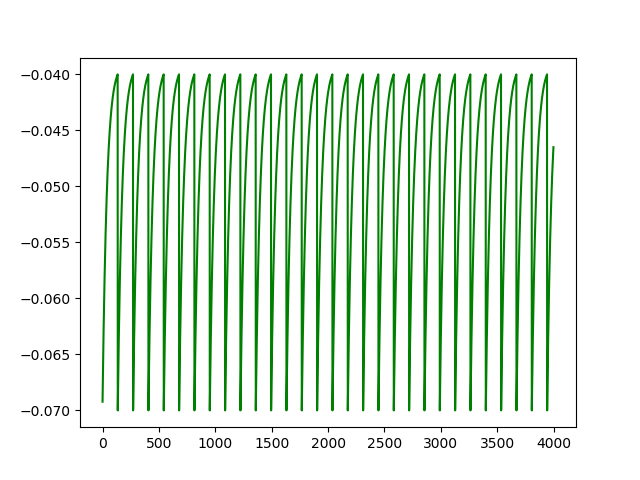
\includegraphics[width=10cm]{graphs/Question1.png}
    \captionof{figure}{Integrate Spike }
\end{center}

\subsection*{Question2}
\begin{center}
    \begin{minipage}{\linewidth} 
    \begin{minipage}{0.45\linewidth}
      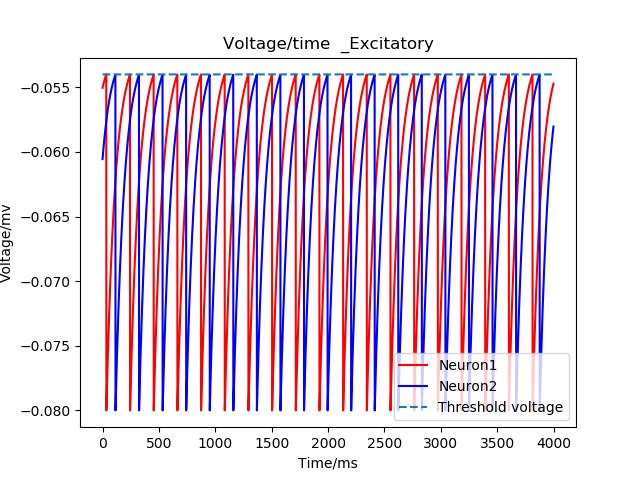
\includegraphics[width=7cm]{graphs/Question2_Excitatory.png}
      \captionof{figure}{Two neurons Excitatory} 
    \end{minipage}
    \hspace{0.05\linewidth}
    \begin{minipage}{0.45\linewidth}
      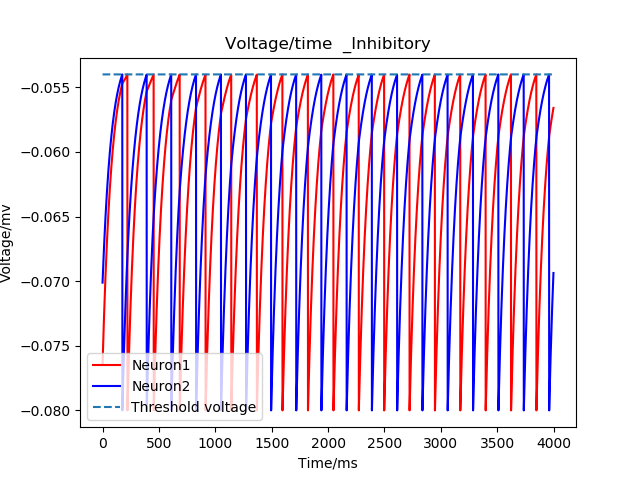
\includegraphics[width=7cm]{graphs/Question2_Inhibitory.png}
      \captionof{figure}{Two neurons Inhibitory}
    \end{minipage}
  \end{minipage} 
\end{center}
\par The left graph shows that two neurons have excitatory synaptic connections
    between each other, and the right is the inhibitory one. 
    Excitatory synaptic connection graph  shows that two neurons tend to synchronize.
    While in inhibitory connection, two neurons have different impulse times. 
    In the same time, One is impulse, and another is calm.                         
\newpage
\subsection*{COMSM2127}
\begin{enumerate}[1)]
\item  
  \par $I_e = (V_{th}-E_L)/R_m$
  \par the minimal current to produce an action potential  $I_e = 3nA$

\item
  \begin{center} 
    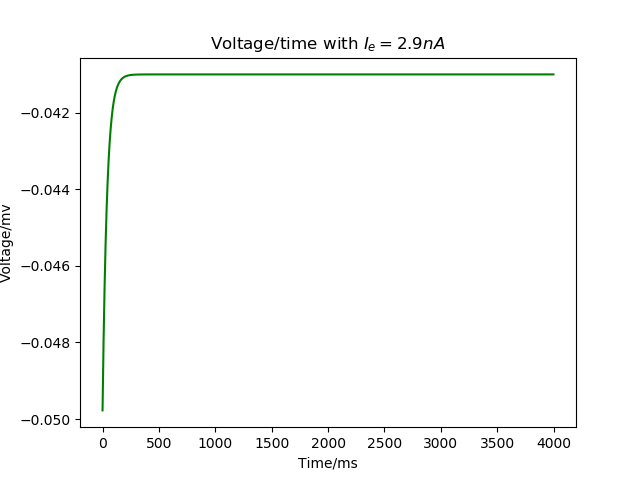
\includegraphics[width=10cm]{graphs/COMS2127_2.png}
    \captionof{figure}{Integrate Spike }
  \end{center}

\item
  \begin{center} 
    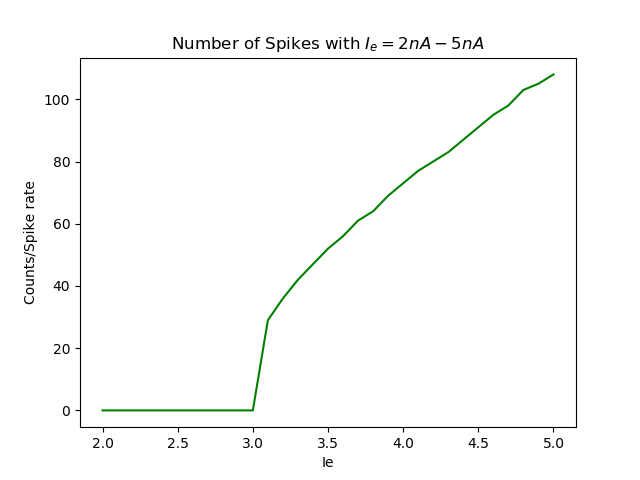
\includegraphics[width=10cm]{graphs/COMS2127_3.png}
    \captionof{figure}{Integrate Spike }
  \end{center}

\end{enumerate}

\newpage

\section*{PartB}
\subsection*{Question 1}
  \begin{center} 
    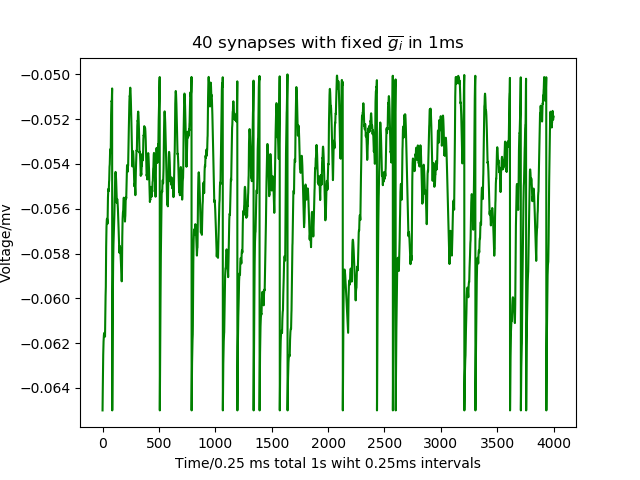
\includegraphics[width=10cm]{graphs/PartB_Question1.png}
    \captionof{figure}{Integrate Spike }
  \end{center}
\par Neuron firing irregularly at a rate of roughly 20 Hz

\subsection*{Question 2}
\par 1) The Figuer 7 shows the synaptic strength distribution converge towards 
at normal distribution shape which center at nearly 2nS. And figure 8 illustrate
the average firing rate of the postsynaptic neuron as a function of time (300s).
The Spike rate is stable at around 1Hz after a Convergence stage.

\par 2) The average value of synaptic weight is around 2.0435 nS. In the last 30 seconds,
STDP-on mode 's fire rate is around at 1Hz, while in STDP-Off mode, the spike rate is around zero.
Just one spike in last 30s for STDP-off mode generally.
\begin{center}
  \begin{minipage}{\linewidth} 
  \begin{minipage}{0.45\linewidth}
    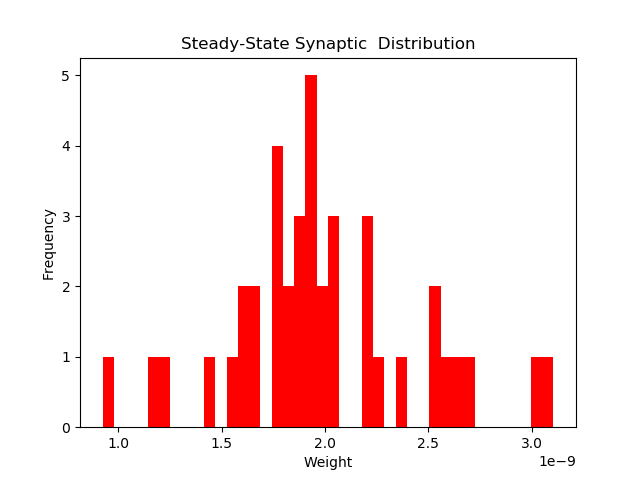
\includegraphics[width=7cm]{graphs/PartB_Question2_STDP_Average_g_6_times.png}
    \captionof{figure}{Steady-State synaptic weight with STDP on} 
  \end{minipage}
  \hspace{0.05\linewidth}
  \begin{minipage}{0.45\linewidth}
    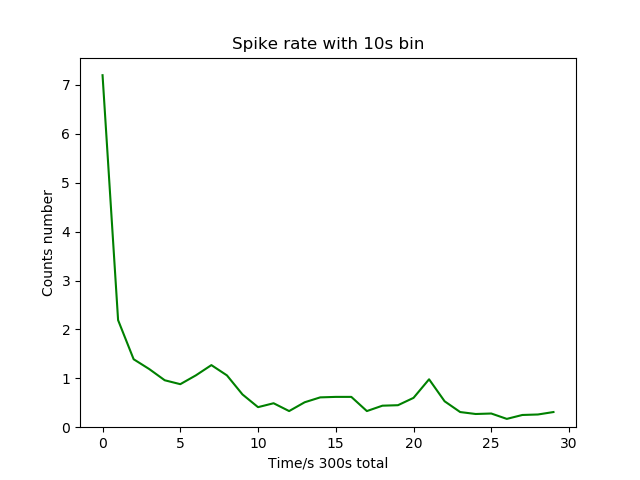
\includegraphics[width=7cm]{graphs/PartB_Question2_STDP_Average_Fire_Rate.png}
    \captionof{figure}{Steady-State spike fire rate with STDP on}
  \end{minipage}
\end{minipage} 
\end{center}

\newpage
\subsection*{Question 3}
\par The figure 9 shows the STDP on mode between 10 and 20Hz,it generally declines  with the increasing input frequency.
And there are some sudden growth point. 
However, figure 10 illusrates that the STDP off mode has an upward trend with increasing input frequency.
Because, the higher input frequency makes the S increase directly, and g is constant in STDP-off mode.
So that, the post-neuron can spike more.
\begin{center}
  \begin{minipage}{\linewidth} 
  \begin{minipage}{0.45\linewidth}
    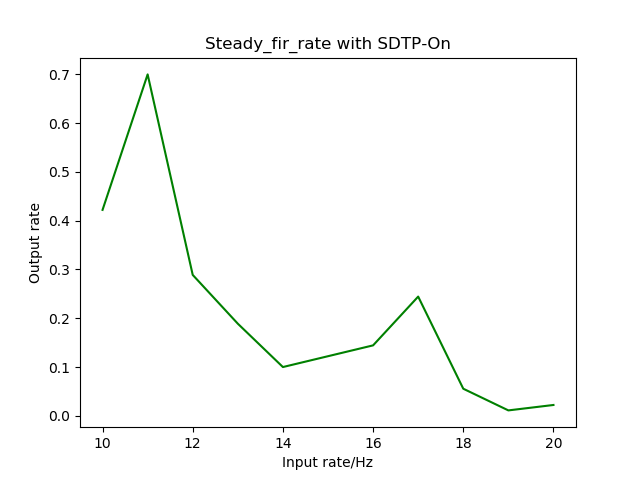
\includegraphics[width=7cm]{graphs/PartB_Question3_10_20Hz_SDTP_On.png}
    \captionof{figure}{Fire rate with STDP On: input 10-20Hz} 
  \end{minipage}
  \hspace{0.05\linewidth}
  \begin{minipage}{0.45\linewidth}
    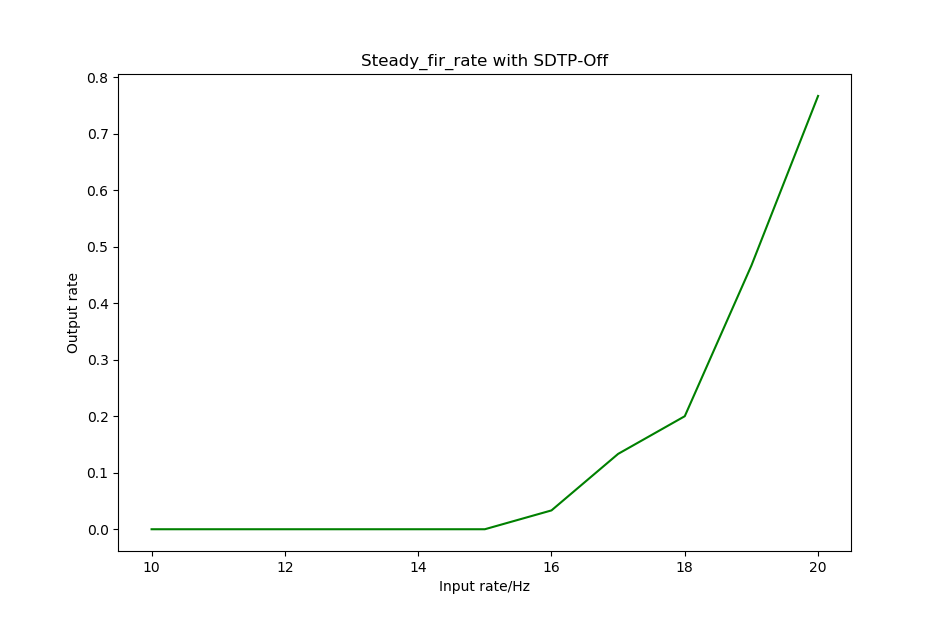
\includegraphics[width=7cm]{graphs/PartB_Question3_10_20Hz_SDTP_Off.png}
    \captionof{figure}{Fire rate with STDP Off: input 10-20Hz}
  \end{minipage}
\end{minipage} 
\end{center}

\par The figure 11 and figure 12 shows the steady-state synaptic strength distribution for r = 10 Hz and r = 20 Hz for the ‘STDP on’ case.
The higher input frequency 's synaptic weights distribution is more even than lower input frequency.
The reason could be that higer input frequency makes more pre-synaptic spike. As the 40 pre-synaptic has the same possion process.
Their distribution is more even.
\begin{center}
  \begin{minipage}{\linewidth} 
  \begin{minipage}{0.45\linewidth}
    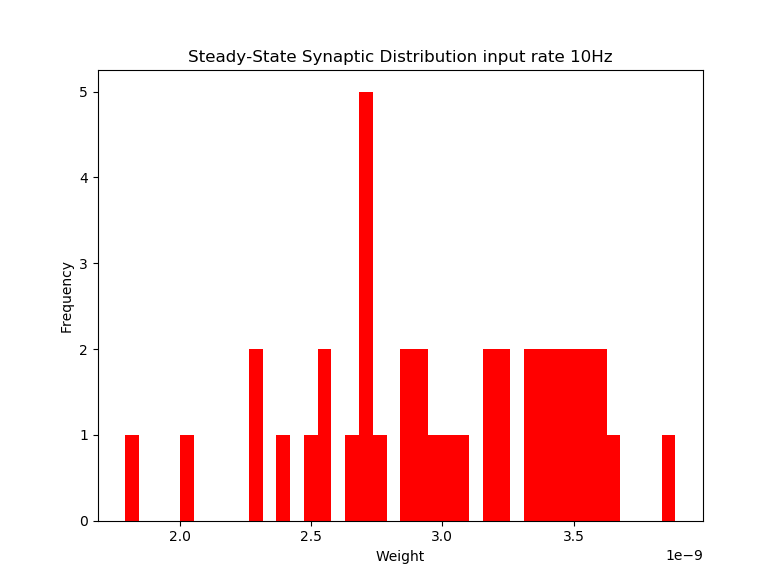
\includegraphics[width=7cm]{graphs/PartB_Question3_10Hz_hism.png}
    \captionof{figure}{Fire rate with STDP On: input 10 Hz} 
  \end{minipage}
  \hspace{0.05\linewidth}
  \begin{minipage}{0.45\linewidth}
    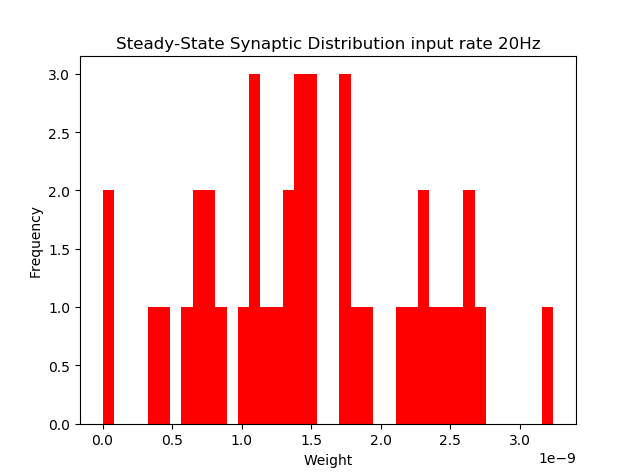
\includegraphics[width=7cm]{graphs/PartB_Question3_20Hz_hism.png}
    \captionof{figure}{Fire rate with STDP On: input 10 Hz}
  \end{minipage}
\end{minipage} 
\end{center}

\newpage
\subsection*{Question 4}
\par The high degree of correlation (B is high) means that steady-state synaptic weights will be also temporally correlated.


\par The figure the mean and standard deviation of the steady-state synaptic strengths as a function of B.
The green line is mean, while red line is std. There has been a decline in the mean of weight.
And the Std is relatively stable and slightly increased, this means that the weight of the synapse is less balanced.

\begin{center} 
  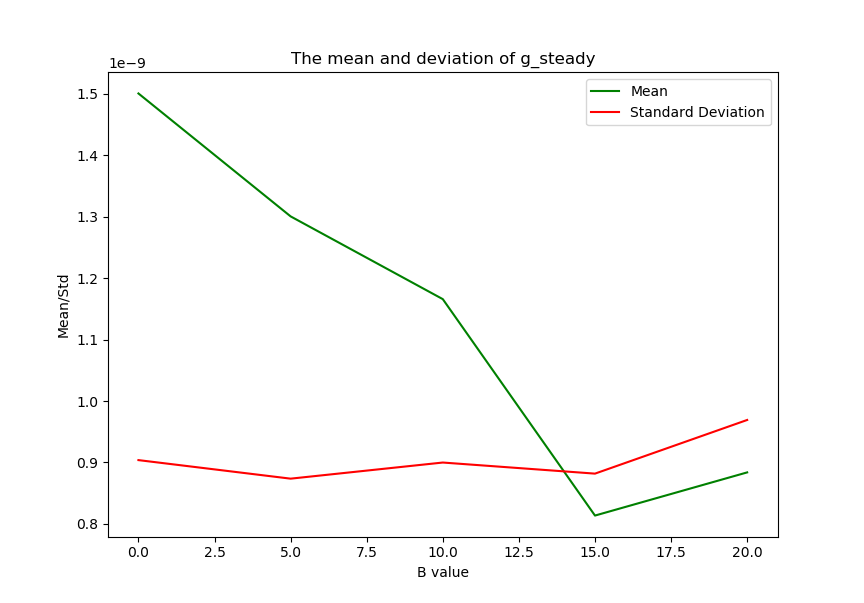
\includegraphics[width=10cm]{graphs/PartB_Question4_mean_g_std_r.png}
  \captionof{figure}{Integrate Spike }
\end{center}

\par B=0 means input frequency is fixed, and small standard deviation
it is becasue, in 300s, each synapse has the same possion (same active probability)
But for B=20, the synapse face different possion process in different time.
The probability is variant, When the post-protrusion is activated, the frequently activated pre-synapse has a larger weight value.
\begin{center}
  \begin{minipage}{\linewidth} 
  \begin{minipage}{0.45\linewidth}
    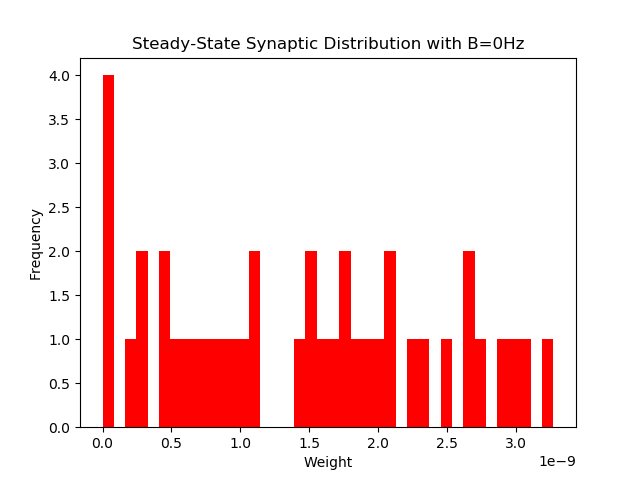
\includegraphics[width=7cm]{graphs/PartB_Questio4_B_0Hz.png}
    \captionof{figure}{Steady-State synaptic weights with B = 0} 
  \end{minipage}
  \hspace{0.05\linewidth}
  \begin{minipage}{0.45\linewidth}
    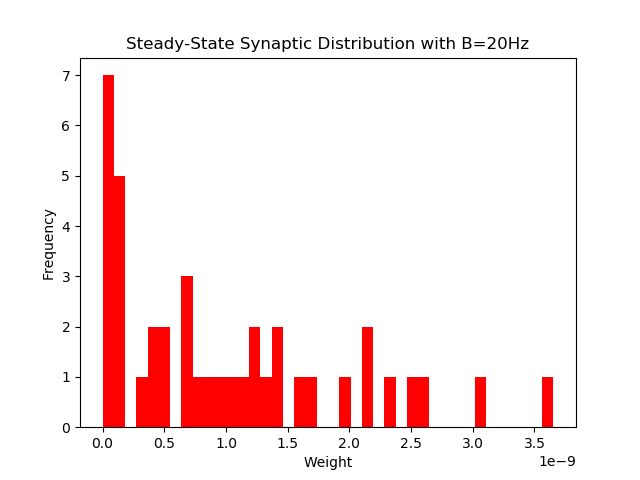
\includegraphics[width=7cm]{graphs/PartB_Questio4_B_20Hz.png}
    \captionof{figure}{Steady-State synaptic weights with B = 20}
  \end{minipage}
\end{minipage} 
\end{center}

\newpage
\subsection*{COMSM2127}
The plot is like the bell shape with the tallest in the middle, decreasing on both sides.
\begin{center} 
  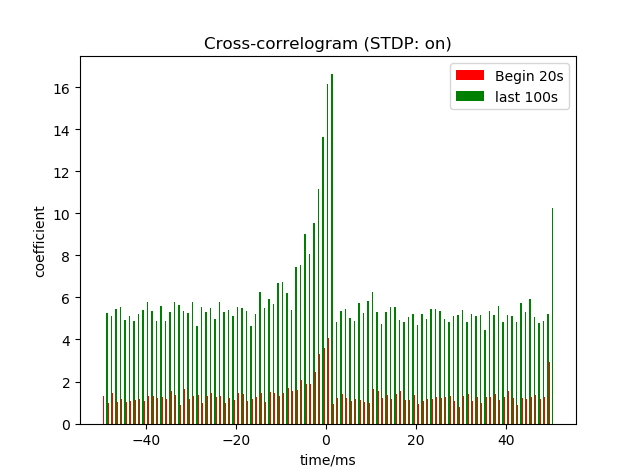
\includegraphics[width=10cm]{graphs/ParB_Cmos2.png}
  \captionof{figure}{cross-correlogram for both cases (start and end of the simulation) }
\end{center}

\end{document}



